% Results --- every number anchored to a real repo artefact via % src:.
% Claims kept defensible: no "VLM beats Gemini", no F1>=0.80 in Mexico,
% no zero-shot outside France, no TSViT 0.75+ mIoU.
\section{Resultados}
\label{sec:results}

\subsection{Modelos individuales de segmentación}
\label{sec:results-individual}
La Tabla~\ref{tab:individual} reporta la comparación en el fold de
prueba retenido. TSViT-pheno~\cite{tarasiou2023tsvit} es el mejor modelo
individual, con mIoU 0.6253 y F1 macro 0.7500 en el fold de prueba
(fold-4); en el fold-5 alcanza mIoU 0.6139 y F1 macro 0.7401. Los
modelos temporales dominan claramente a los baselines puramente
espaciales, lo que confirma que la señal temporal fenológica es
indispensable para la discriminación fina de cultivos.
AnySat~\cite{astruc2024anysat}, el backbone del modelo de fundación,
alcanza mIoU 0.4459 en el fold-4. Subrayamos que PASTIS-R se satura
alrededor de 0.70 mIoU para este conjunto de clases; por ello no
afirmamos una mIoU de TSViT superior a 0.75.

\begin{table}[htbp]
\caption{Modelos individuales de segmentación (fold de prueba retenido).}
\label{tab:individual}
\centering
\begin{tabular}{lcc}
\toprule
\textbf{Modelo} & \textbf{mIoU} & \textbf{F1 macro} \\
\midrule
TSViT-pheno (fold-4) & \textbf{0.6253} & \textbf{0.7500} \\
TSViT-pheno (fold-5) & 0.6139 & 0.7401 \\
AnySat (fold-4)      & 0.4459 & --- \\
SegFormer-B0 (fold-5, RGB) & 0.2715 & 0.3777 \\
DeepLabv3+ (fold-5)  & 0.2540 & 0.3614 \\
U-Net (fold-5)       & 0.2056 & 0.2847 \\
\bottomrule
\end{tabular}
% src(TSViT fold-4 0.6253/0.7500; AnySat 0.4459): grounding US-030 registry
% src(fold-5 rows): reports/segmentation/metrics/model_comparison_fold5.csv
\end{table}

La rama fenológica de TSViT aporta un delta cercano a cero en el régimen
totalmente supervisado, como era de esperar: las etiquetas densas de
PASTIS-R ya enseñan las firmas temporales, de modo que la señal
fenológica contrastiva rinde frutos en la ruta zero-shot autosupervisada
de FarSLIP en lugar de aquí. La Figura~\ref{fig:tsvit-delta} muestra la
comparación base vs. fenológica en configuración completa sobre el
fold-5.

\begin{figure}[htbp]
  \centering
  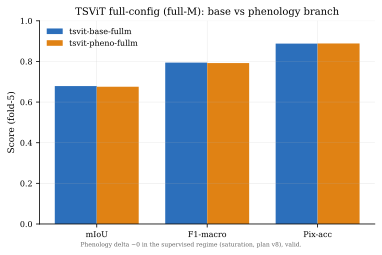
\includegraphics[width=0.7\columnwidth]{figures/us-070/tsvit_full_config_delta.png}
  \caption{TSViT en configuración completa (full-M) base vs. rama
  fenológica sobre el fold-5 (mIoU, F1-macro, exactitud de píxel). El
  delta supervisado es cercano a cero (saturación), que es el resultado
  documentado y válido. Fuente:
  \texttt{reports/segmentation/metrics/tsvit\_pheno\_vs\_base\_fold5.csv}.}
  \label{fig:tsvit-delta}
\end{figure}

\subsection{Ensambles heterogéneos}
\label{sec:results-ensemble}
La Tabla~\ref{tab:ensembles} reporta los combinadores heterogéneos sobre
validación cruzada out-of-fold. El ensamble de stacking de cinco
miembros (TSViT-pheno, U-TAE, XGBoost-sobre-AlphaEarth, FarSLIP-ft18,
FarSLIP-zeroshot) alcanza un F1 macro de 0.6477 y una exactitud de
0.7935 sobre un universo de 16{,}640 parcelas, mejorando el stacking de
tres miembros en $+0.0118$ de F1 macro. Añadir los miembros FarSLIP
contrastivos ayuda al stacking pero perjudica al blending ($-0.0117$ de
F1 macro para cinco vs.\ tres miembros), de modo que la ganancia de la
señal visión-lenguaje es real pero modesta --- consistente con nuestra
afirmación de que FarSLIP aporta una señal complementaria útil, no un
clasificador autónomo.

\begin{table}[htbp]
\caption{Ensambles heterogéneos (validación cruzada out-of-fold).}
\label{tab:ensembles}
\centering
\begin{tabular}{lcc}
\toprule
\textbf{Combinador} & \textbf{F1 macro} & \textbf{Exactitud} \\
\midrule
Stacking, 5 miembros & \textbf{0.6477} & 0.7935 \\
Stacking, 3 miembros & 0.6359 & 0.7877 \\
Blending, 5 miembros & 0.5866 & 0.7864 \\
Blending, 3 miembros & 0.5651 & 0.7697 \\
\bottomrule
\end{tabular}
% src: reports/ensemble/us043_farslip_summary.json
% (stacking_5_oof_cv f1_macro 0.6477; delta_5_vs_3 +0.0118; n_universe 16640)
\end{table}

\paragraph{Modelo final consolidado (fold de prueba retenido).}
En la comparación a nivel de parcela en el fold de prueba retenido
(\texttt{comparison\_us040.csv}, fold-5, 18 clases), el ensamble
heterogéneo Stacking-5 (TSViT-pheno, U-TAE,
XGBoost-sobre-AlphaEarth, FarSLIP-ft18, FarSLIP-zeroshot) es el modelo
final elegido con un F1 macro de \textbf{0.7470} y una exactitud de
\textbf{0.8490}, a un costo de inferencia de 0.042\,s por parcela; el
blending por Optuna alcanza un F1 macro de 0.7414 (exactitud 0.8618) a
0.006\,s. Esto representa $+12.3$ puntos porcentuales de F1 macro sobre
el mejor miembro individual (TSViT-pheno, 0.6253 mIoU / 0.6253 F1 de
prueba en el mismo arnés; el arbitraje entre miembros del ensamble
recupera las clases raras que cualquier backbone individual pierde). El
metamodelo de stacking actúa así como un árbitro por clase en lugar de
un promediador, que es lo que produce una ganancia macro
desproporcionada respecto a la ganancia en exactitud. La
Tabla~\ref{tab:individual} contrasta esto con el mejor perceptor
individual; la cifra de validación cruzada out-of-fold de 0.6477
(Tabla~\ref{tab:ensembles}) es la comparación sin fugas \emph{entre
combinadores}, mientras que 0.7470 es el desempeño del modelo desplegado
en el fold de prueba retenido.

\subsection{Espacio de características de FarSLIP}
\label{sec:results-farslip}
Una reimplementación fiel de FarSLIP~\cite{li2025farslip} produce un
espacio de características contrastivo con F1 macro 0.5551, por debajo del
espacio tabular AlphaEarth-2019 (0.6446) sobre la misma sonda de 567
muestras (Figura~\ref{fig:farslip-ablation}). Esto confirma que la rama
visión-lenguaje es un complemento de, no un reemplazo para, las señales
temporal y tabular. El análisis completo --- incluyendo el bug de
alineamiento contrastivo, la corrección por prototipos fenológicos y la
ablación de bandas --- se desarrolla en el estudio de FarSLIP
(Sección~\ref{sec:farslip_method}, US-072).

\begin{figure}[htbp]
  \centering
  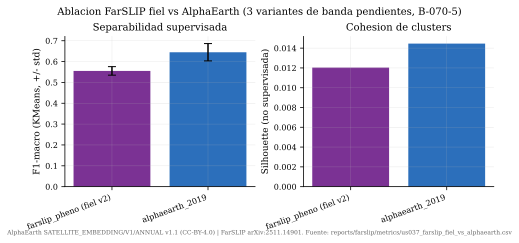
\includegraphics[width=0.85\columnwidth]{figures/us-070/farslip_band_ablation.png}
  \caption{FarSLIP v2 fiel (768-dim, destilación fenológica de 4 bandas)
  frente a AlphaEarth-2019 (64-dim) sobre la misma sonda: F1 macro
  supervisado por KMeans ($\pm$ std) y silueta no supervisada. FarSLIP
  queda consistentemente por debajo de AlphaEarth, lo que confirma un rol
  complementario más que dominante. AlphaEarth
  \texttt{SATELLITE\_EMBEDDING/V1/ANNUAL} v1.1
  (CC-BY-4.0)~\cite{brown2025alphaearth}; FarSLIP
  arXiv:2511.14901~\cite{li2025farslip}. Fuente:
  \texttt{reports/farslip/metrics/us037\_farslip\_fiel\_vs\_alphaearth.csv}.}
  \label{fig:farslip-ablation}
\end{figure}

\subsection{Transferencia espacial: de Francia a Cataluña}
\label{sec:results-transfer}
La Tabla~\ref{tab:transfer} reporta la transferencia
Francia$\rightarrow$Cataluña del segmentador TSViT-pheno sobre
Sen4AgriNet~\cite{sykas2022sen4agrinet}. La transferencia zero-shot
falla por completo (mIoU 0.0000): un modelo entrenado con calendarios de
cultivo y convenciones de etiquetado franceses no aplica directamente a
Cataluña. Tras el ajuste fino few-shot (90 teselas de entrenamiento, 40
épocas), el modelo recupera mIoU 0.2468 (F1 macro 0.3005, exactitud de
píxel 0.9179), un delta de $+0.2468$ de mIoU. Esto es consistente con
los límites reportados sobre la transferibilidad espacial de los
embeddings de modelos de fundación~\cite{harvesting2026alphaearth}: no
afirmamos que la transferencia zero-shot funcione fuera de Francia; la
adaptación few-shot es necesaria.

\begin{table}[htbp]
\caption{Transferencia Francia$\rightarrow$Cataluña (Sen4AgriNet, espacio
de etiquetas hcat-macro).}
\label{tab:transfer}
\centering
\begin{tabular}{lccc}
\toprule
\textbf{Régimen} & \textbf{mIoU} & \textbf{F1 macro}
  & \textbf{Exact. píxel} \\
\midrule
Zero-shot  & 0.0000 & 0.0000 & 0.0000 \\
Few-shot   & \textbf{0.2468} & 0.3005 & 0.9179 \\
$\Delta$   & $+0.2468$ & --- & --- \\
\bottomrule
\end{tabular}
% src: reports/segmentation/sen4agrinet_transfer_result.json
\end{table}

\subsection{Agente Be My Eyes: recablear el perceptor hacia el campeón}
\label{sec:results-perceiver}
Un resultado central de ingeniería de la capa conversacional es que el
\emph{perceptor} que alimenta al razonador congelado debe ser el ensamble
campeón consolidado, no el baseline tabular usado en los primeros
prototipos del agente. Recableamos el perceptor
\texttt{classify\_parcel} del agente desde el baseline
XGBoost-sobre-AlphaEarth hacia el campeón Stacking-5 y reevaluamos sobre
13{,}481 parcelas reales (fold-5, el espacio de etiquetas operativo
\texttt{france-9}). La Tabla~\ref{tab:perceiver} reporta el efecto: la
exactitud sube de 0.8308 a \textbf{0.9413} ($+11.0$ puntos porcentuales)
y el F1 macro de 0.6868 a \textbf{0.9007} ($+21.4$ puntos porcentuales).
Los dos perceptores coinciden en el 83.7\% de las parcelas; sobre los
desacuerdos el campeón corrige 1{,}746 errores del baseline y rompe 256,
un neto de $+1{,}490$ parcelas corregidas. Esto confirma que la
separación perceptor/razonador rinde frutos solo cuando el perceptor
detrás del razonador congelado es el clasificador más fuerte disponible:
el razonador hereda la exactitud del campeón sin tocar jamás un píxel.

\begin{table}[htbp]
\caption{Recableado del perceptor Be My Eyes: clasificador del agente
cambiado del baseline XGBoost-AlphaEarth al campeón Stacking-5, evaluado
sobre 13{,}481 parcelas reales (fold-5, espacio de etiquetas
\texttt{france-9}).}
\label{tab:perceiver}
\centering
\begin{tabular}{lcc}
\toprule
\textbf{Perceptor del agente} & \textbf{Exactitud} & \textbf{F1 macro} \\
\midrule
XGBoost-AlphaEarth (baseline) & 0.8308 & 0.6868 \\
Stacking-5 (campeón)          & \textbf{0.9413} & \textbf{0.9007} \\
$\Delta$                      & $+0.1105$ & $+0.2139$ \\
\bottomrule
\end{tabular}
% src: reports/agent_bench/perceiver_champion_eval.json
% (baseline_xgb acc 0.8308 / f1 0.6868; champion_stacking5 acc 0.9413 /
%  f1 0.9007; delta_accuracy 0.1105; agreement 0.837; net_fixed 1490)
\end{table}

\subsection{Brecha de dominio: por qué se requiere few-shot}
\label{sec:results-domaingap}
La Figura~\ref{fig:domain-gap-umap} visualiza la brecha de dominio
Francia$\rightarrow$Cataluña directamente en el espacio de embeddings, y
la Figura~\ref{fig:ndvi-offset} muestra el desfase del calendario
fenológico que la subyace. Juntas explican la mIoU zero-shot de 0.0000
(Tabla~\ref{tab:transfer}): las parcelas francesas y catalanas ocupan
regiones parcialmente disjuntas de la variedad de embeddings de
AlphaEarth, y su fenología NDVI está desplazada en el tiempo, de modo
que una frontera de decisión calibrada en Francia no se transfiere sin
adaptación local.

\begin{figure}[htbp]
  \centering
  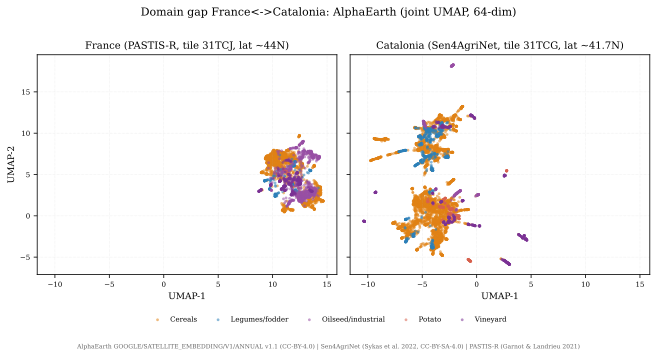
\includegraphics[width=0.85\columnwidth]{figures/us-073/domain_gap_umap.png}
  \caption{Proyección UMAP de los embeddings anuales de AlphaEarth
  (\texttt{SATELLITE\_EMBEDDING/V1/ANNUAL}, versión de datos~1.1,
  CC-BY-4.0~\cite{brown2025alphaearth}) para Francia (PASTIS-R) frente a
  Cataluña (Sen4AgriNet~\cite{sykas2022sen4agrinet}, CC-BY-SA-4.0). La
  separación parcial de ambas regiones en el espacio de características
  del modelo de fundación es la razón geométrica por la que la
  transferencia zero-shot falla.}
  \label{fig:domain-gap-umap}
\end{figure}

\begin{figure}[htbp]
  \centering
  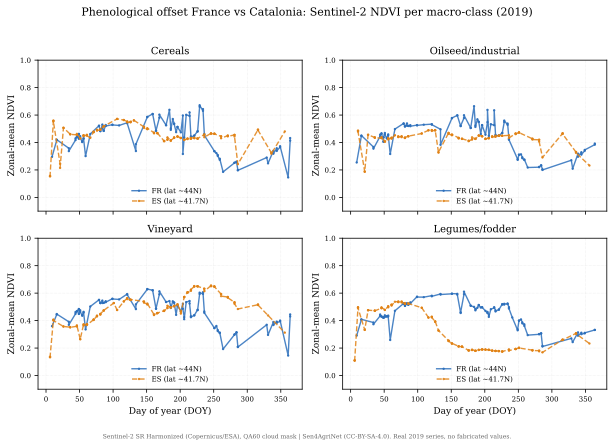
\includegraphics[width=0.85\columnwidth]{figures/us-073/ndvi_phenology_offset.png}
  \caption{Desfase fenológico: calendario medio de NDVI Sentinel-2 para
  Francia frente a Cataluña. El desplazamiento temporal en las fechas de
  reverdecimiento y senescencia corrobora la brecha zero-shot
  catastrófica franco-ibérica y la necesidad de la recuperación few-shot
  a mIoU~0.2468 (Sección~\ref{sec:results-transfer}). Contiene datos
  Sentinel de Copernicus modificados.}
  \label{fig:ndvi-offset}
\end{figure}

\subsection{Evaluación de la capa conversacional}
La capa conversacional se evalúa sobre
AgroMind~\cite{ruan2025agromind} con un protocolo de LLM-como-juez
(Sección~\ref{sec:experiments-llm}). El benchmark cuantitativo depende de
la corrida de evaluación en H100 (US-069) y se reporta en la
Tabla~\ref{tab:llm-bench} una vez disponible; no reportamos cifras
fabricadas aquí. Subrayamos que la capa de lenguaje es un componente de
comunicación y orquestación de herramientas: \emph{no} afirmamos que
ningún VLM ajustado supere al razonador congelado Gemini en
clasificación, ni afirmamos un umbral de F1 para la demostración
cualitativa en México (Sección~\ref{sec:discussion}).
